\chapter{Teaching Your PI Controller to Behave (Part I)}

Richard Poley manages the training activities for our C2000 microcontrollers (MCUs), and co-teaches the TI Industrial Control Seminar series with me.  (If you have never attended one of Richard’s classes on control theory, you are really missing a spectacular treat!)  One of the stories Richard likes to tell is how the PI(D) controller was invented.  To paraphrase, a Russian-American engineer named Nicolas Minorsky was designing automatic steering systems for the US Navy in the early 1920s by observing how a helmsman steered a ship under different conditions.  According to Wikipedia.org, he noticed that the actions of the helmsman could be approximated by a simple amplification of the error signal under calm conditions, but this simple model was inadequate to describe the helmsman’s response during a steady disturbance like a stiff gale.  This finally led to the addition of an integral term to correct for continuous steady-state errors.  Later, the derivative term was added to improve controllability even further.

Continuing with the Wikipedia.org narrative, test trials of his automatic steering system based on a PI controller were first carried out on the \textit{USS New Mexico}.  After some adjustments, he was able to control the angular error to less than two degrees.  When the D term was added, the error improved to within one sixth of a degree, which was better than what most helmsmen could achieve manually!  Minorsky published his findings (also in the early 1920s), but like most famous inventions, few engineers took notice at the time.  However, we know today that his discovery launched a new era in the design of control systems!

\begin{figure}[H]
    \centering
    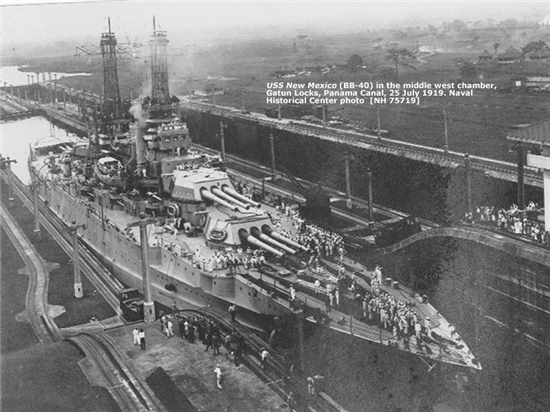
\includegraphics[width=\linewidth]{01/01_uss_new_mexico}
    \caption{\textit{U.S.S. New Mexico around the time it was retrofitted with PID control}}
    \label{fig:01ussnewmexico}
\end{figure}


    One of the questions I invariably am asked during our Industrial Control seminars is “How do you tune a PI controller?”  I typically fumble for some Bode plots or throw some simulation data up on the screen to show that the process is somewhat empirical, and very subjective to the kind of response for which you are looking.  This usually results in some disappointed stares from the audience as they realize that all I did was dodge the question instead of answering it.

After a recent seminar, I decided that I needed a better answer, so I started investigating this topic in earnest.  What I discovered changed my thinking about PI controllers!  I now believe that designing and tuning PI control loops (regardless of whether they are speed loops or current loops) is much more deterministic than I had thought!  Granted, there are still plenty of degrees of freedom depending on what kind of response you are looking for, as well as an endless litany of subtle variations on the basic PI structure itself.  But by following a few basic rules, you should be able to tune your PI loop without needing a PhD.

But first, the small print.  My analysis is limited to loads having only real poles.  If your design has prominent complex poles resulting from excessive torsional resonance between the motor and load, then the controller will have to be more sophisticated than a simple PI structure anyway to cancel the resonance effects.  But in most cases, a stiff shaft coupler should tame the torsional resonance to the point where the use of a standard PI control structure is acceptable.  Also, throughout most of this blog series I assume that the load has no viscous damping.

So, what do you think of when you hear the phrase “PI controller?”  For many, it is the conventional parallel path topology shown below.  The error signal is split into two separate paths: one which is directly amplified, and the other is amplified and then integrated.  The amplified error signal and the integrated error signal are then recombined at the output via a simple addition operation.  The integrator is included to drive the steady-state error of the system to zero, since any non-zero steady-state error will theoretically result in a boundless integrator output.  While the integrator plays a crucial role in the operation of the PI controller, it also brings a nasty set of headaches with it.  For example, let’s say that the error in your control loop is zero, which means the controlled signal is equal to the commanded signal.  Now add a small offset to the controlled signal and watch what happens.  Since the error signal is no longer zero, the integrator output will start growing …and growing …and growing in an attempt to null the error signal again.

Now remove the offset and watch what happens.  The controlled signal will eventually return to the commanded value once again, but not right away.  The integrator output is still very large, which causes the controlled signal to wildly overshoot the commanded value while the integrator output is “dumped.”  During this time, the profile of the “controlled” signal is not controlled at all, and may even result in damage to your system if not constrained.  It’s kind of like winding up a spring tightly and then suddenly releasing it.  That’s why this effect in PI controllers is called “windup.”  There are many ways to mitigate the windup effect, but most techniques involve some sort of limiting of the integrator’s output.  We will discuss this in more detail later in this series.

\begin{center}
    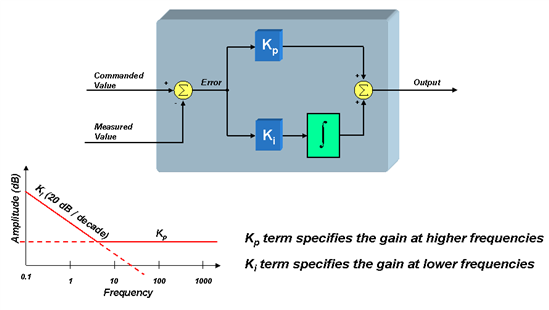
\includegraphics[width=1\linewidth]{01/02}
\end{center}

While the PI topology is fairly easy to understand, the deep dark secret is “how do you set the values for $K_p$ and $K_i$?”  This has been the subject for much debate, and it is rather difficult to intuitively understand the effect that each term has on your motor control system.  The $K_p$ term sets the high frequency gain of the control loop, as shown above.  The $K_i$ term sets the low frequency gain, and theoretically has infinite gain at DC.  The frequency which delineates the high frequencies from the low frequencies is referred to as the “zero” of the controller and corresponds to the inflection point in the frequency plot.  But we are still no closer to understanding how to set the controller’s coefficients.  So most engineers simply resort to the tried and true technique of "hit or miss."

Another popular form of the PI controller (and the one we will use for our analysis) is the “series” topology which is shown below.

\begin{center}
    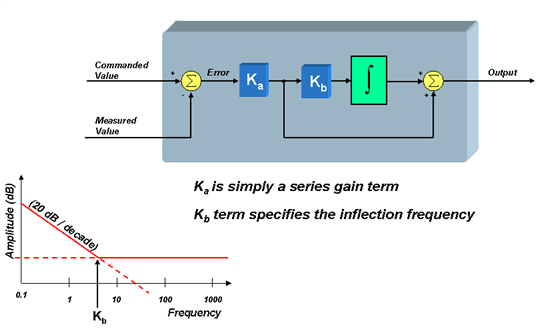
\includegraphics[width=1\linewidth]{01/03}
\end{center}

From this diagram, we can see that the relationship between the two sets of coefficients is defined as follows:

\begin{align*}
    K_a &= K_p \\
    K_b &= \frac{K_i}{K_p}
\end{align*}

But notice that in this structure, $K_a$ sets the gain for ALL frequencies, and $K_b$ directly defines the inflection point (zero) of the controller in \unit{\radian\per\second}.  Both forms are pretty much equal in terms of software implementation.  However, many engineers prefer the series form over the parallel form since $K_a$ and $K_b$ directly correlate to tangible system parameters.  It’s pretty easy to understand the effect that $K_a$ has on the controller’s performance, since it sets the gain in your open-loop transfer function.  But what is the system significance of the zero inflection point?  This is one of the discoveries I made, which I want to share with you in my next blog.  In the meantime\dots

Keep Those Motors Spinning,\\

\includegraphics[width=0.2\linewidth]{01/04_dave}
\vfill
\textit{Feb 28 2013 15:21 PM}


